See 
\tabref{tab:std-conic-params-sol}
and 
\figref{fig:11/11/2/1Fig1}.
	\probref{prob:conic-params} was used to obtain the conic and directrix parameters.
			The latus recturm is obtained using \eqref{eq:latus-ellipse}
			
\begin{figure}[H]
		\begin{center}
	%	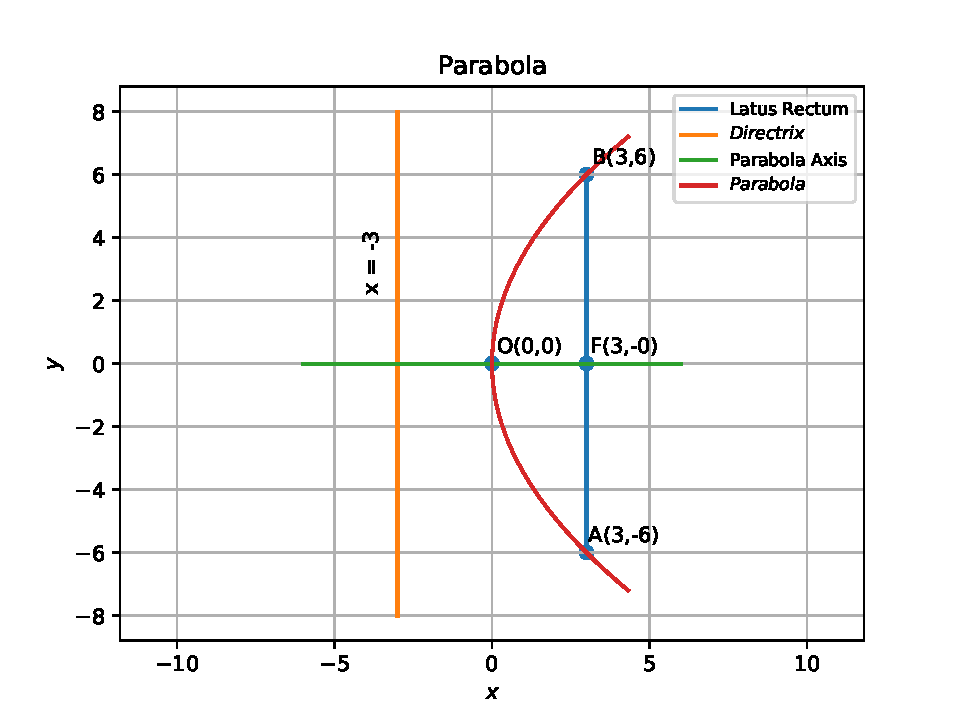
\includegraphics[width=0.75\columnwidth]{chapters/11/11/2/1/figs/problem1.pdf}
	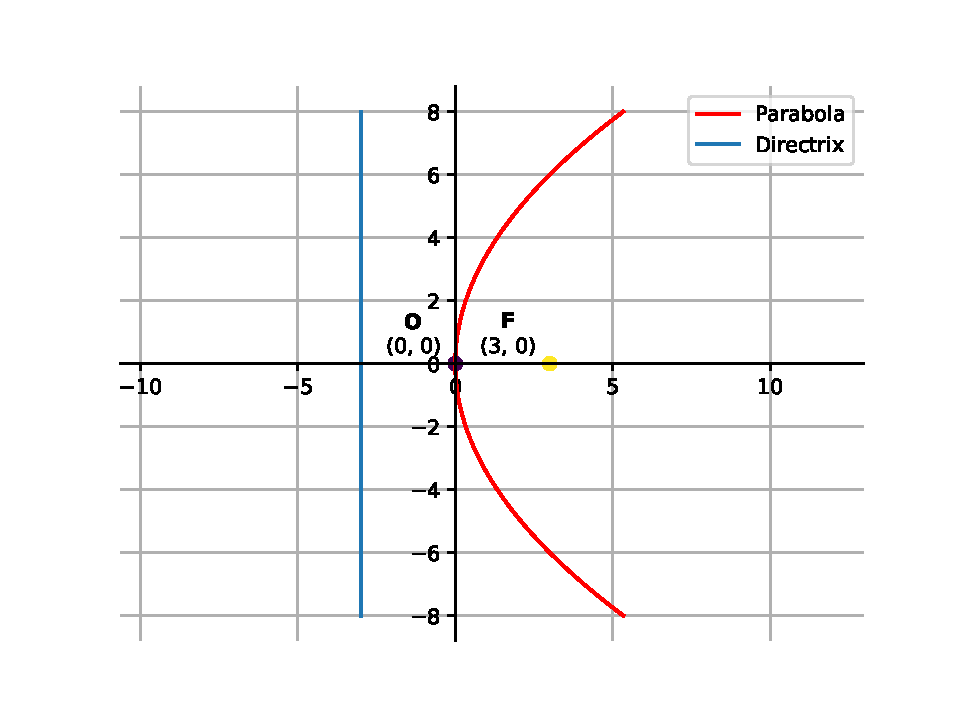
\includegraphics[width=0.75\columnwidth]{chapters/11/11/2/1/figs/fig.pdf}
	\end{center}
\caption{}
\label{fig:11/11/2/1Fig1}
\end{figure}
